\documentclass[compress,t,11pt]{beamer}
%\documentclass[handout,compress,t,11pt]{beamer}  % don't build out slides
\usetheme[sectionpage=none]{metropolis}           % Use metropolis theme
%\useinnertheme{circles} 
%\usefonttheme{structurebold}
\usefonttheme{serif}
\definecolor[named]{Gray}{RGB}{111,112,114}
\definecolor[named]{DarkGray}{RGB}{48,48,48}
\definecolor[named]{Cardinal}{RGB}{179,22,34}
\usepackage[T1]{fontenc}
\usepackage[altbullet]{lucidabr}
\usepackage{textcomp}
\usepackage{upquote} % needed to make straight quotes work in listings
\usepackage{listgolang}
\usepackage{mathtools}
\usepackage{comment}
\usepackage{tikz}
\usetikzlibrary{trees,shapes,plotmarks,arrows,er,automata,petri,topaths,positioning}
\usepackage{pifont}
\usepackage{clrscode}
\usepackage{setspace}
\usepackage{multirow}
\usepackage{array}

% In theory, but it breaks here
%\usepackage[symbol]{footmisc}
%\renewcommand{\thefootnote}{\fnsymbol{footnote}}

% 1   asterisk    *       2   dagger  †       3   double dagger   ‡
% 4   section symbol  §   5   paragraph   ¶   6   parallel lines  \\
% 7   two asterisks   **  8   two daggers ††  9   two double daggers  ‡‡

\setbeamercolor{palette primary}{fg=white,bg=Cardinal}
\setbeamercolor{palette secondary}{fg=white,bg=Gray}
\setbeamercolor{palette tertiary}{fg=white,bg=Cardinal}
\setbeamercolor{palette quaternary}{fg=white,bg=Gray}
\setbeamercolor{palette sidebar primary}{fg=white,bg=Cardinal}
\setbeamercolor{palette sidebar secondary}{fg=white,bg=Gray}
\setbeamercolor*{titlelike}{fg=Cardinal}
\setbeamercolor{structure}{fg=Gray}
\setbeamercolor{title separator}{fg=Cardinal}
\setbeamercolor{alerted text}{fg=Cardinal}

\newcommand{\card}[1]{\ensuremath{\left|#1\right|}}
\newcommand{\norm}[1]{\ensuremath{\|#1\|}}

\title[Go Concurrency]{\bf Concurrency in Go}
\author{Matt Holiday} 
\institute[CP]{Cardinal Peak}
\date{9 January 2019}
\subtitle{{\it ``Don't communicate by sharing memory; \\
instead, share memory by communicating''}}
% \defbeamertemplate*{headline}{split theme}{}
% \setbeamertemplate{navigation symbols}{}
% \setbeamertemplate{frametitle}{\color{Cardinal}\bfseries\vskip 6pt\insertframetitle}
%\titlegraphic{\hfill\includegraphics[width=.25\textwidth,height=.25\textheight]{cp-logo-2x.png}}
\titlegraphic{
\begin{tikzpicture}[overlay, remember picture,scale=0.4]
\node[at=(current page.north east), anchor=north east] (a) {};
\node[below left = 0.1cm and 0.1cm of a] (b)
{\includegraphics[width=.25\textwidth,height=.25\textheight]{cp-logo-2x.png}};
% \node[below left=2.56cm and 2.9cm of b]
% {\includegraphics[width=.1\textwidth]{go-logo.png}};
\end{tikzpicture}}

\setbeamerfont{footline}{series=\bfseries\selectfont}
\setbeamersize{text margin left=12pt,text margin right=12pt}
\linespread{1.0}
\metroset{block=fill}

\begin{document}
\begin{frame}[plain]
\titlepage
\end{frame}

\section{Introduction}
\begin{frame}[fragile]
    \frametitle{What's the problem?}
    \only<1-3>{We want to find duplicate files based on their {\bf content} \par}
    \vspace{\baselineskip}
    \only<2-3>{Use a secure hash, because the names / dates may differ \par}
    \vspace{2\baselineskip}
% can't use verbatim inside only or really even in a frame
\defverbatim{\hashes}{\footnotesize\begin{verbatim}
f088913 2
    /Users/mholiday/Dropbox/Emergency/FEMA_P-320_2014_508.pdf
    /Users/mholiday/Dropbox/Emergency/nps61-072915-01.pdf
\end{verbatim}}
    \only<2-3>{\hashes}
    \vspace{1\baselineskip}
    \only<3-3>{It takes nearly {\bf 5 minutes} to comb through my Dropbox folder \par}
    % can we illustrate a hash table to a list of files ...
\end{frame}

\section{Serial Approach}
\begin{frame}[fragile]
    \frametitle{How it works: Declarations}
\begin{golang}
package main

import (
    "crypto/md5"
    "fmt"
    "io"
    "log"
    "os"
    "path/filepath"
)

type pair struct {
	hash string
	path string
}

type fileList []string
type results  map[string]fileList
\end{golang}

\end{frame}
\begin{frame}[fragile]
    \frametitle{How it works: Hashing}
\begin{golang}
func hashFile(path string) pair {
	file, err := os.Open(path)

	if err != nil && err != os.ErrNotExist {
		log.Fatal(err)
	}

	defer file.Close()

	hash := md5.New() // fast & good enough

	if _, err := io.Copy(hash, file); err != nil {
		log.Fatal(err)
	}

	return pair{fmt.Sprintf("%x", hash.Sum(nil)), path}
}
\end{golang}
\end{frame}

\begin{frame}[fragile]
    \frametitle{How it works: Searching}
\begin{golang}
func searchTree(dir string) (results, error) {
	hashes := make(results)

	err := filepath.Walk(dir, func(p string, fi os.FileInfo,
                                   err error) error {
        // ignore the error parm for now

		if fi.Mode().IsRegular() && fi.Size() > 0 {
			h := hashFile(p)
			hashes[h.hash] = append(hashes[h.hash], h.path)
		}

		return nil
	})

	return hashes, err
}
\end{golang}
\end{frame}

\begin{frame}[fragile]
    \frametitle{How it works: Output}
\begin{golang}
func main() {
    if len(os.Args) < 2 {
        log.Fatal("Missing parameter, provide dir name!")
    }

    if hashes, err := searchTree(os.Args[1]); err == nil {
    	for hash, files := range hashes {
    		if (len(files) > 1) {
                // we will use just 7 chars like git
    			fmt.Println(hash[len(hash)-7:], len(files))

    			for _, file := range files {
    				fmt.Println("   ", file)
    			}
    		}
    	}
    }
}
\end{golang}
\end{frame}

\section{Concurrent Approach \#1}
\begin{frame}
    \frametitle{A concurrent approach (like map-reduce)}
    Use a fixed pool of goroutines and a collector and channels \par

    \begin{center}
        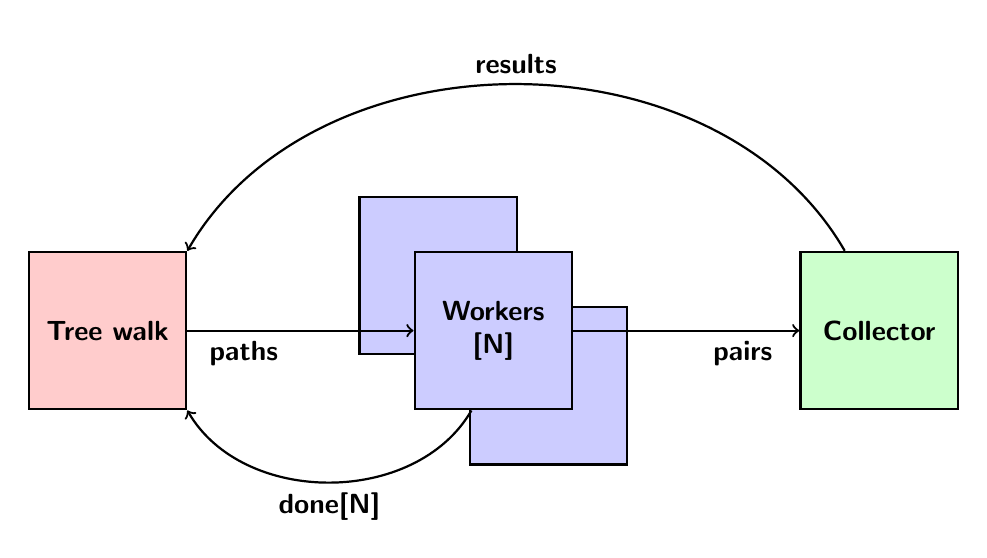
\begin{tikzpicture}[scale=0.7]            
            \tikzstyle{state}=[rectangle,minimum size=2cm,font=\sffamily\bfseries,draw]
            \tikzstyle{link}=[font=\sffamily\bfseries]

            \tikzstyle{every edge}=[thick,draw]

            \tikzstyle{M}=[state,thick,fill=green!20]    % main graph
            \tikzstyle{C}=[state,thick,fill=blue!20]     % clique
            \tikzstyle{A}=[state,thick,fill=red!20]      % key node

            \node[A] (0) at (-1, 0) {Tree walk};
            \node[C] (1) at ( 5, 1) {};
            \node[C] (1) at ( 7,-1) {};
            \node[C] (1) at ( 6, 0) [align=center]{Workers\\ {[N]}};
            \node[M] (2) at (13, 0) {Collector};

            \tikzstyle{E}=[ultra thick,color=red]  % min cut

            \path[->] (0) edge node[link,below,near start] {paths} (1);
            \path[->] (1) edge node[link,below,near end]   {pairs} (2);
            \path[->] (1) edge [bend left=60]  node[link,below] {done[N]} (0.south east);
            \path[->] (2) edge [bend right=60] node[link,above] {results} (0.north east);
        \end{tikzpicture}
    \end{center}
\end{frame}

\begin{frame}[fragile]
    \frametitle{How it works: Collecting the hashes}
\begin{golang}
func collectHashes(pairs <-chan pair, result chan<- results) {
	hashes := make(results)

	for p := range pairs {
		hashes[p.hash] = append(hashes[p.hash], p.path)
	}

	result <- hashes
}
\end{golang}
\end{frame}

\begin{frame}[fragile]
    \frametitle{How it works: Replacing the processor}
\begin{golang}
func processFiles(paths <-chan string, pairs chan<- pair,
                  done chan<- bool) {
	for path := range paths {
		pairs <- hashFile(path)
	}

	done <- true
}
\end{golang}
\end{frame}

\begin{frame}[fragile]
    \frametitle{How it works: Replacing the tree walk}
\begin{golang}
workers := 2 * runtime.GOMAXPROCS(0)

paths := make(chan string)
pairs := make(chan pair)
done := make(chan bool)
result := make(chan results)

for i := 0; i < workers; i++ {
	go processFiles(paths, pairs, done)
}

// we need another goroutine so we don't block here

go collectHashes(pairs, result)

. . .
\end{golang}
\end{frame}

\begin{frame}[fragile]
    \frametitle{How it works: Replacing the tree walk}
\begin{golang}
err := filepath.Walk(dir, func(p string, fi os.FileInfo,
                               err error) error {
	// again, ignore the error passed in

	if fi.Mode().IsRegular() && fi.Size() > 0 {
		paths <- p
	}

	return nil
})

if err != nil {
    log.Fatal(err)
}

// we must close the paths channel so the workers stop
close(paths)
. . .
\end{golang}
\end{frame}

\begin{frame}[fragile]
    \frametitle{How it works: Replacing the tree walk}
\begin{golang}
. . .

// wait for all the workers to be done

for i := 0; i < workers; i++ {
	<-done
}

// by closing pairs we signal that all the hashes
// have been collected; we have to do it here AFTER
// all the workers are done

close(pairs)

hashes := <-result

return hashes
\end{golang}
\end{frame}

\begin{frame}
    \frametitle{Evaluation \#1}
    \only<1-4>{56.11s in the version shown above \par}
    \vspace{\baselineskip}
    \only<2-4>{52.76s with a buffer to {\tt pairs} \par}
    \vspace{\baselineskip}
    \only<3-4>{Buffering {\tt pairs} keeps the workers working \par}
    \vspace{2\baselineskip}
    \only<4-4>{51.36s with twice as many workers \par}
\end{frame}

\section{Concurrent Approach \#2}
\begin{frame}
    \frametitle{Another concurrent approach}
    \only<1-5>{Add a goroutine for each directory in the tree \par}
    \vspace{\baselineskip}
    \only<2-5>{This improves the performance slightly, we're not waiting
               on paths to be identified \par}
    \vspace{2\baselineskip}
    \only<3-5>{51.14s in the basic version \par}
    \vspace{\baselineskip}
    \only<4-5>{50.03 adding buffers on channels to/from workers \par}
    \vspace{\baselineskip}
    \only<5>{48.75 with twice as many workers}
\end{frame}

\begin{frame}[fragile]
    \frametitle{How it works: Parallel tree walk}
\begin{golang}
. . .

wg := new(sync.WaitGroup)

// multi-threaded walk of the directory tree; we need a
// waitGroup because we don't know how many to wait for

wg.Add(1)
err := walkDir(dir, paths, wg)

if err != nil {
	log.Fatal(err)
}

wg.Wait()
close(paths)

. . .
\end{golang}
\end{frame}

\begin{frame}[fragile]
    \frametitle{How it works: Parallel tree walk}
\begin{golang}
func walkDir(dir string, paths chan<- string,
             wg *sync.WaitGroup) error {
	defer wg.Done()

	visit := func(p string, fi os.FileInfo, err error) error {
		// ignore the error passed in

        // ignore dir itself to avoid an infinite loop!
		if fi.Mode().IsDir() && p != dir {
			wg.Add(1)
			go walkDir(p, paths)
			return filepath.SkipDir
		}

        . . .
\end{golang}
\end{frame}

\begin{frame}[fragile]
    \frametitle{How it works: Parallel tree walk}
\begin{golang}
        . . .

		if fi.Mode().IsRegular() && fi.Size() > 0 {
			paths <- p
		}

		return nil
	}

	return filepath.Walk(dir, visit)
}
\end{golang}
\end{frame}

\section{Concurrent Approach \#3}
\begin{frame}
    \frametitle{The final approach: Goroutines galore!}
    \only<1-5>{Use a goroutine for every directory and file hash \par}
    \vspace{\baselineskip}
    \only<2-5>{Without some controls, we'll run out of threads! \par}
    \vspace{2\baselineskip}
    \only<3-5>{We'll limit the number of {\bf active} goroutines instead \par}
    \vspace{\baselineskip}
    \only<4-5>{46.93s using 32 workers was the best time \par}
    \vspace{\baselineskip}
    \only<5>{Adding more workers actually makes the time grow longer }
\end{frame}

\begin{frame}
    \frametitle{Channels as counting semaphores}
    \only<1-3>{A goroutine can't proceed without sending on the channel \par}
    \vspace{2\baselineskip}
    \only<2-3>{The buffer provides a fixed upper bound (unlike a WaitGroup) \par}
    \vspace{2\baselineskip}
    \only<3-3>{One goroutine can start for each one that quits \par}
    % illustrate this with a queue and a cloud of goroutines
    % animate one ending and another starting up
\end{frame}

\begin{frame}
    \frametitle{What that looks like}
    \begin{center}
        \begin{tikzpicture}[remember picture,overlay,scale=0.7]
            \tikzset{shift={(current page.center)},xshift=0cm,yshift=-0.75cm}
            \tikzstyle{state}=[rectangle,minimum size=2cm,font=\sffamily\bfseries,draw]
            \tikzstyle{link}=[font=\sffamily\bfseries]
            \tikzstyle{link1}=[font=\sffamily\itshape]

            \tikzstyle{every edge}=[thick,draw]

            \tikzstyle{M}=[state,thick,fill=green!20]    % main graph
            \tikzstyle{C}=[state,thick,fill=blue!20]     % clique
            \tikzstyle{A}=[state,thick,fill=red!20]      % key node

            \node[A] (0) at (-7, 0) {Main};
            \node[C] (3) at (-1, 1) {};
            \node[C] (4) at ( 1,-1) {};
            \node[C] (1) at ( 0, 0) [align=center]{Workers\\ {[*]}};
            \node[M] (2) at ( 7, 0) {Collector};

            \tikzstyle{E}=[ultra thick,color=red]  % min cut

            \path[dashed,->] (0) edge node[link1,below,near start]                 {starts}    (1);
            \path[->]        (1) edge node[link,below,near end]                    {pairs}     (2);
            \path[->]        (1) edge[out=30,in=150,looseness=10] node[link,below] {limits[N]} (1);
            \path[->]        (2) edge [bend left=60] node[link,above]              {results}   (0.south east);
        \end{tikzpicture}
    \end{center}
\end{frame}
            % \path[->] (1.west) edge [bend right=90] node[link,below left] {limits[N]} (4.south);

\begin{frame}[fragile]
    \frametitle{How it works: Limiting goroutines}
\begin{golang}
// we don't need a channel for paths or to signal done but
// we need a buffered channel to act as a counting semaphore

wg := new(sync.WaitGroup)
limits := make(chan bool, workers)
pairs := make(chan pair, workers)
result := make(chan results)

go collect(pairs, result)

. . .
\end{golang}
\end{frame}

\begin{frame}[fragile]
    \frametitle{How it works: Limiting goroutines}
\begin{golang}
. . .

wg.Add(1)
err := walkDir(dir, pairs, wg, limits)

if err != nil {
	log.Fatal(err)
}

wg.Wait()
close(pairs)

hashes := <-result

return hashes
\end{golang}
\end{frame}

\begin{frame}[fragile]
    \frametitle{How it works: Modified processing}
\begin{golang}
func processFile(path string, pairs chan<- pair,
                 wg *sync.WaitGroup, limits chan bool) {
    defer wg.Done()

	limits <- true

	defer func() {
		<-limits		
	}()

	pairs <- hashFile(path)
}
\end{golang}
\end{frame}

\begin{frame}[fragile]
    \frametitle{How it works: Modified tree walk}
\begin{golang}
func walkDir(dir string, pairs chan<- pair, wg *sync.WaitGroup,
             limits chan bool) error {
	defer wg.Done()

	visit := func(p string, fi os.FileInfo, err error) error {
		// ignore the error passed in

		if fi.Mode().IsDir() && p != dir {
			wg.Add(1)
			go walkDir(p, pairs, wg, limits)
			return filepath.SkipDir
		}

		. . .
\end{golang}
\end{frame}

\begin{frame}[fragile]
    \frametitle{How it works: Modified tree walk}
\begin{golang}
        . . .

		if fi.Mode().IsRegular() && fi.Size() > 0 {
			wg.Add(1)
			go processFile(p, pairs, wg, limits)
		}

		return nil
	}

	limits <- true

	defer func() {
		<-limits
	}()

	return filepath.Walk(dir, visit)
}
\end{golang}
\end{frame}

\begin{frame}
    \frametitle{Go gotchas 1: Deadlock}
    A goroutine is {\bf preemptible} only when it starts a (non-inlined)
    function call, blocks on a channel or mutex, or makes a blocking system call.
    \vspace{\baselineskip}
\begin{alertblock}{Potential Problems}
    If your goroutine isn't preemptible, garbage collection will never run,
    because it must first ``stop the world.''
\end{alertblock}
    \vspace{\baselineskip}
    However, if the {\tt main()} function exits, all goroutines terminate.
\end{frame}

\begin{frame}[fragile]
    \frametitle{Go gotchas 1: Deadlock}
\begin{golang}
go func() {
    var i byte

    for i = 0; i <= 255; i++ {
        // infinite loop does nothing
        // doesn't get elided
        // and can't be preempted
    }
}()

runtime.Gosched()    // yield execution
runtime.GC()         // force GC

// DEADLOCK

fmt.Println("Done")  // never happens
\end{golang}
\end{frame}

\begin{frame}[fragile]
    \frametitle{Go gotchas 1: Deadlock Fixed}
\begin{golang}
go func() {
    var i byte

    for i = 0; i <= 255; i++ {
        // infinite loop does nothing
        // doesn't get elided

        // but we can yield
		if (i == 123) {
			runtime.Gosched()
		}
    }
}()

runtime.Gosched()    // yield execution
runtime.GC()         // force GC
fmt.Println("Done")  // prints Done
\end{golang}
\end{frame}

\begin{frame}[fragile]
    \frametitle{Go gotchas 2: Closure capture}
    A closure shouldn't capture a {\bf mutating} variable, e.g. a loop index. \par
    \vspace{0.6\baselineskip}
    If it does, it will get the wrong value! \par
    \vspace{0.2\baselineskip}
\begin{golang}
for i := 0; i < 10; i++ {   // WRONG
    go func() {
        fmt.Println(i)
    }()
}
\end{golang}
    Instead, \alert{pass the variable's value as a parameter}.
    \vspace{0.2\baselineskip}
\begin{golang}
for i := 0; i < 10; i++ {  // RIGHT
    go func(i int) {
        fmt.Println(i)
    }(i)
}
\end{golang}
\end{frame}

\begin{frame}[fragile]
\frametitle{Channel state reference}
{\renewcommand{\arraystretch}{1.5}
\begin{table}[h!]
  \begin{center}
    \begin{tabular}{l||l|l|l}%{m{2.5cm}||m{1.6cm}|m{1.6cm}|m{3.5cm}}
      \textbf{State} & \textbf{Receive}  & \textbf{Send} & \textbf{Close}\\
      \hline\hline
      Nil & Block* & Block* & Panic \\
      \hline
      Empty & Block & Write & Close \\
      \hline
      Partly Full & Read & Write & \multirow{2}{*}{Readable until empty} \\
      \cline{1-3}
      Full & Read & Block \\
      \hline
      Closed & Default Value** & \multicolumn{2}{c}{Panic} \\
      \hline\hline
      Receive-only & OK & \multicolumn{2}{c}{Compile Error} \\
      \hline
      Send-only & Compile Error & \multicolumn{2}{c}{OK} \\
    \end{tabular}
  \end{center}
\end{table}
}
{\footnotesize
  * \verb|select| ignores a nil channel since it would always block \\
  ** Reading a closed channel returns \verb|(<default-value>, !ok)|
}
\end{frame}
\end{document}